% Workflow figure (report Section 2). Built by report/make_workflow_figure.py.
\documentclass[tikz,border=1pt]{standalone}
\usepackage[scaled=0.92]{helvet}
\renewcommand{\familydefault}{\sfdefault}
\usepackage{amssymb}
\usetikzlibrary{positioning,arrows.meta,calc}

\definecolor{content}{HTML}{2F6DB5}
\definecolor{motion}{HTML}{E07B39}
\definecolor{ink}{HTML}{2B2F36}
\definecolor{muted}{HTML}{6B7280}
\definecolor{panel}{HTML}{F4F6F9}
\definecolor{rule}{HTML}{CDD3DB}
\definecolor{unet}{HTML}{AEB6C2}

\newcommand{\fw}{0.6}   % thumbnail side (cm)
% \strip{x}{y}{prefix}{border colour}: three frames, top-left corner at (x,y)
\newcommand{\strip}[4]{%
  \foreach \i in {0,1,2}{%
    \node[inner sep=0, anchor=north west] at ({#1+\i*(\fw+0.04)},#2)
      {\includegraphics[width=\fw cm]{#3_\i.png}};}
  \draw[#4, line width=0.7pt, rounded corners=0.5pt] (#1-0.03,#2+0.03) rectangle ({#1+3*\fw+0.11},{#2-\fw-0.03});}

\begin{document}
\begin{tikzpicture}[
  font=\scriptsize\color{ink}, >={Stealth[length=1.8mm]},
  pnl/.style={fill=panel, draw=rule, rounded corners=3pt, line width=0.4pt},
  tag/.style={circle, fill=ink, text=white, font=\scriptsize\bfseries, inner sep=1.2pt, minimum size=3.6mm},
  title/.style={anchor=west, font=\footnotesize\bfseries\color{ink}},
  sub/.style={anchor=north west, inner sep=0, font=\scriptsize\bfseries\color{muted}},
  body/.style={anchor=north west, align=left, text width=#1, inner sep=0, font=\scriptsize\color{ink}},
  lab/.style={anchor=south west, inner sep=0},
  chip/.style={draw=rule, fill=white, rounded corners=2pt, align=left, text width=2.5cm,
               inner sep=2.5pt, minimum height=0.8cm, font=\scriptsize\color{ink}},
  flow/.style={->, draw=ink, line width=0.6pt}]

% ---------------------------------------------------------------- panels
\fill[pnl] (0,0) rectangle (3.75,6.2);
\fill[pnl] (4.25,0) rectangle (10.2,6.2);
\fill[pnl] (10.7,0) rectangle (16.5,6.2);
\node[tag] at (0.3,5.9) {a};     \node[title] at (0.5,5.9) {Framing and pilots};
\node[tag] at (4.55,5.9) {b};    \node[title] at (4.75,5.9) {Locating content and motion};
\node[tag] at (11.0,5.9) {c};    \node[title] at (11.2,5.9) {Intervening and editing};

% ---------------------------------------------------------------- (a)
\node[sub] at (0.2,5.45) {Problem};
\node[draw=rule, fill=white, rounded corners=2pt, anchor=north west, text width=3.15cm, inner sep=3pt,
      align=left] at (0.2,5.15)
  {``a \textcolor{content}{\textbf{golden retriever}} \textcolor{motion}{\textbf{running}} on a beach''\\[2pt]
   \textcolor{content}{$\blacksquare$} content: what is shown\\
   \textcolor{motion}{$\blacktriangle$} motion: how it moves};
\node[sub] at (0.2,3.65) {Planning};
\node[body=3.35cm] at (0.2,3.35)
  {model: AnimateDiff\\
   3 hypotheses with their tests,\\
   fixed before any data};
\node[sub] at (0.2,2.2) {Pilot experiments};
\node[body=3.35cm] at (0.2,1.9)
  {94\,s and 10.2\,GB per clip\\
   pixel motion follows the shape\\
   87.9\,GiB of activations per clip\\
   $\Rightarrow$ score pairs while generating};

% ---------------------------------------------------------------- (b)
\node[sub] at (4.45,5.45) {One-word-swap pairs};
\node[lab] at (4.45,4.95) {anchor: athlete walking};
\strip{4.45}{4.9}{anchor}{ink}
\node[lab, text=content] at (4.45,3.95) {subject swap: \textbf{soldier}};
\strip{4.45}{3.9}{subject}{content}
\node[lab, text=motion] at (4.45,2.95) {verb swap: \textbf{jumping}};
\strip{4.45}{2.9}{verb}{motion}

% U-Net glyph: encoder bars shrink, decoder bars grow; dots = hooks
\begin{scope}[shift={(6.85,3.6)}]
  \foreach \h [count=\k from 0] in {1.5,1.1,0.75,0.45}{
    \fill[unet] ({\k*0.13},{-\h/2}) rectangle ++(0.09,\h);
    \fill[unet] ({1.24-\k*0.13},{-\h/2}) rectangle ++(0.09,\h);
    \fill[motion] ({\k*0.13+0.045},{\h/2+0.08}) circle (0.028);
    \fill[motion] ({1.24-\k*0.13+0.045},{\h/2+0.08}) circle (0.028);}
  \fill[unet] (0.53,-0.15) rectangle ++(0.27,0.3);
  \fill[motion] (0.665,0.23) circle (0.028);
  \node[align=center, font=\scriptsize\color{muted}] at (0.665,-1.15) {U-Net, 25 steps\\95 hooks};
\end{scope}
\draw[flow] (6.45,4.6) -- (6.8,3.85);
\draw[flow] (6.45,3.6) -- (6.8,3.6);
\draw[flow] (6.45,2.6) -- (6.8,3.35);

% selectivity map (rows down0 ... up3, columns steps 0 ... 24)
\def\mx{8.65} \def\my{4.5} \def\mw{1.4} \def\mh{1.8}
\node[anchor=north west, inner sep=0] at (\mx,\my)
  {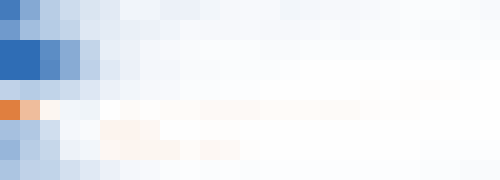
\includegraphics[width=\mw cm, height=\mh cm]{smap.png}};
\draw[rule] (\mx,\my) rectangle ++(\mw,-\mh);
\draw[ink, line width=0.8pt] (\mx,{\my-5*\mh/9}) rectangle ++({3*\mw/25},{-\mh/9});
\node[anchor=south, inner sep=1.5pt] at ({\mx+\mw/2},\my) {selectivity map};
\node[rotate=90, anchor=south, inner sep=1pt, font=\scriptsize\color{muted}] at (\mx,{\my-\mh/2}) {layer};
\node[anchor=north, inner sep=1.5pt, font=\scriptsize\color{muted}] at ({\mx+\mw/2},{\my-\mh}) {step 0 $\to$ 24};
\draw[flow] (8.15,3.6) -- (8.4,3.6);

\node[body=5.6cm] at (4.45,1.75)
  {\textcolor{motion}{$\blacktriangle$ \textbf{motion}}: one decoder block, first 2--3 steps (boxed)\\
   \textcolor{content}{$\blacksquare$ \textbf{content}}: almost every layer};
\node[body=5.6cm, text=muted] at (4.45,0.95)
  {360 clips $\cdot$ 750 pairs $\cdot$ 3 hypotheses $\cdot$ linear probes};

% ---------------------------------------------------------------- (c)
\node[sub] at (10.9,5.45) {Swap motion and appearance};
\node[lab] at (10.9,4.95) {A: athlete walking};
\strip{10.9}{4.9}{anchor}{motion}
\node[lab] at (10.9,3.95) {B: soldier jumping};
\strip{10.9}{3.9}{b}{content}
\node[draw=ink, fill=white, rounded corners=2pt, align=center, inner sep=2.5pt, text width=1.0cm]
  (op) at (13.62,4.1) {lockstep\\edit};
\draw[flow, motion] (12.9,4.6) -- (op.west |- 0,4.25);
\draw[flow, content] (12.9,3.6) -- (op.west |- 0,3.95);
\node[lab] at (14.45,4.95) {edit: soldier,};
\node[lab] at (14.45,4.68) {A's walk};
\strip{14.45}{4.62}{edit}{ink}
\draw[flow] (op.east) -- (14.38,4.1);
\node[body=5.4cm, align=center, text=muted] at (10.9,3.1)
  {patch the frame mean or the frame-varying part,\\or inject temporal attention};

\node[chip, anchor=north west] at (10.9,2.55) {\textbf{Selection, then test}\\pick on 4 dev pairs,\\test on 12 held-out};
\node[chip, anchor=north west] at (13.72,2.55) {\textbf{Motion LoRAs}\\placed by the map};
\node[chip, anchor=north west] at (10.9,1.4)  {\textbf{Other models}\\4 model variants};
\node[chip, anchor=north west] at (13.72,1.4)  {\textbf{Interface}\\live edit, upload, browse};

% ---------------------------------------------------------------- links between panels
\draw[flow] (3.8,3.1) -- (4.2,3.1);
\draw[flow] (10.25,3.1) -- (10.65,3.1);

% ---------------------------------------------------------------- timeline
\draw[->, muted, line width=0.5pt] (0,-0.35) -- (16.5,-0.35);
\foreach \x/\t in {1.875/Sep, 7.225/20 Oct, 13.6/21--25 Oct}
  {\draw[muted] (\x,-0.28) -- (\x,-0.42); \node[below, font=\scriptsize\color{muted}] at (\x,-0.42) {\t};}
\draw[dashed, muted, line width=0.5pt] (4.0,6.35) -- (4.0,-0.42)
  node[below, font=\scriptsize\color{muted}] {prep review, 21 Sep};
\end{tikzpicture}
\end{document}
